\documentclass{article}

\usepackage{amsmath}
\usepackage{amsfonts}
\usepackage{amssymb}
\usepackage{graphicx}
\usepackage{subcaption}
\usepackage[colorinlistoftodos]{todonotes}
\usepackage[colorlinks=true, allcolors=blue]{hyperref}

\graphicspath{ {figures/} }

% Commands
\newcommand{\alphabet}{\mathcal{A}}


\title{Generative model validation for immune receptor repertoires}
\author{Branden Olson, Software WG folks, Frederick A Matsen IV}


\begin{document}

\maketitle

\begin{abstract}
The adaptive immune system generates an incredible diversity of B cell receptor sequences coding for antibodies that keep dangerous pathogens at bay.
These sequences arise by a complex process of random naive cell generation followed by affinity maturation, yielding considerable latent structure underlying the distribution of sequences.
Probabilistic models formalize our understanding of the random process of immune repertoire generation.
Model benchmarking often consists of simulating from the true model, performing inference on data derived from the simulation, and assessing the accuracy of the inference.
Model validation attempts to delineate the discrepancies between the simulations and observed data sets, which is challenging since the full underlying distribution is unknown.
One can compare such complex data sets to each other and to model simulations using summary statistics, or quantities that summarize some aspect of the repertoires.
Although many models exist, and the realism of these models can be assessed by comparison of summary statistics, a systematic comparison of models to data using these statistics has not yet been done.
In this paper we perform a systematic comparison of existing models to data sets through the lens of summary statistics.
We find regarding the models...
We find regarding the summary statistics...
We have an R package.
\end{abstract}

\section*{Introduction}

B cells and T cells, also known as lymphocytes, play critical roles in adaptive immunity through the cooperative identification of and response to antigens.
The sophisticated rearrangement of the genes that construct B cell receptors (BCRs) and T cell receptors (TCRs) allows for the recognition of a highly diverse set of antigen epitopes.
An individual's immune repertoire is the set of lymphocyte receptors present in the immune system and is constantly changing in time.

The random generation of immune repertoires from gene rearrangements invites probabilistic modeling and in particular model-based simulation.
In particular, it is natural to benchmark model-based inferential tools by applying them to simulations from the assumed model and assessing the performance.
Simulation tools can also be used to generate a null distribution to compare to data to look for a specific effect, such as natural selection \cite{Yaari2012-kk}.

To build and improve on such probabilistic frameworks, we must identify the strengths and limitations of the underlying models.
We usually perform model validation by comparing features of simulated data to observed repertoire samples and evaluating their concordance (or lack thereof).
This is not as easy a task for repertoires as it is for other problems, where a model output may simply be a real number.
In contrast, repertoire models generate sets of nucleotide sequences that are sparse in the very large set of all possible nucleotide sequences.
Moreover, accurate repertoire models incorporate various underyling structures such as clonal family clusters or phylogenetic trees, further compounding the difficulties.
Indeed, immune repertoires are large, complex objects.

In such a setting, summary statistics are useful (and sometimes sufficient) for expressing discrepancies between model simulations and data, and also between simulations and between data sets.
Luckily, researchers have already derived many means of quantifying important features of repertoires.

As noted above, BCR repertoires consist of collections of trees.
Thus, repertoires are substantially more complex than trees, and even for this strictly simpler problem there has been a lot of effort to define good summary statistics \cite{Mooers1997-jl}.
Tree statistics, albeit other ones, have also been a major focus of previous work in BCR sequence analysis \cite{Dunn-Walters2004-hv,Mehr2004-ej,Steiman-Shimony2006-fm,Shahaf2008-cc}.

However, they are more complex, inviting other means of quantifying and comparing them.
See below for a list of them.



A hefty collection of summary statistics for repertoires will be tabulated and discussed in detail below, and range from simple statistics such as the level of GC content, to statistics such as tree shapes which are applied to complex inferences.
Simple statistics acting on raw sequences are helpful because they are robust to potentially problematic assumptions of inferential methods as well as implementation intricacies.
For example, if our inferential method was linear regression, comparing fit slopes is less useful when the data is not close to a line, but comparing nonparametric statistics like the sample mean or range is still sensible.
On the other hand, statistics on the result of estimations are revealing when inferential model fit is reasonable, and can help reduce noise from sampling or measurement error.
In our linear regression example, comparing the general trends of points can be less distracted by noise than comparing the sets of points directly.

[Cartoon of projecting repertoires in various directions into real space, and comparing the resulting projections?]

In this paper, we gather summary statistics on repertoires and use them to perform model validation for state of the art simulation tools against real data.
Our methodology also constitutes a systematic means of comparing any two lymphocyte repertoires, whether experimentally observed or artifically generated.
Furthermore, we investigate the effectiveness of various summary statistics in distinguishing between different observed repertoires as well as between simulated and observed data.
Although by comparing various generative models to real data, we obtain a validated means of generating data for benchmarking inferential tools, we don't do that here.
Also, although summary statistics can be used in simulation-based inferential methods such as approximate Bayesian computation, we don't do that here either.

\section*{Methods}

\subsection*{Repertoire Comparison}

Applications of a methodical lymphocyte repertoire comparison tool include:
\begin{itemize}
\item Comparing simulated repertoires to observed ones (model selection and validation)
\item Contrasting repertoires in the context of antigen response or vaccination design and evaluation
\item Assessing the performance of competing repertoire analysis tools
\item Evaluating artificial lymphocyte repertoires \cite{Finlay2012}
\end{itemize}

\begin{table}
\begin{tabular}{c|c|c|c}
Summary statistic & Annotations & Clustering & Phylogeny
\\
\hline \hline
Pairwise distance matrix & No & No & No \\
Distance to $k$th closest sequence & No & No & No \\
GC-content & No & No & No \\
Hot/cold spot motif frequencies & No & No & No \\
$k$mer frequency & No & No & No \\
\hline
Distance from naive to mature & Yes & No & No \\
Distance to $k$th closest V-sequence & Yes & No & No \\
CDR3 length & Yes & No & No \\
Joint distribution of germline gene use & Yes & No & No \\
Levenshtein distance between CDR3s & Yes & No & No \\
Physiochemical features of CDR3s & Yes & No & No \\
Per-gene substitution rate & Yes & No & No \\
Per-gene-per-position substitution rate & Yes & No & No \\
Base-by-base substitution matrix & Yes & No & No \\
Transition/transversion rates & Yes & No & No \\
Positional distance between mutations & Yes & No & No \\
Distance from naive to mature & Yes & No & No \\
V/D/J deletion/insertion lengths & Yes & No & No \\
Transition matrix for insertions & Yes & No & No \\
\hline
Cluster size distribution & Yes & Yes & No \\
Hill numbers (diversity indices) & Yes & Yes & No \\
Selection estimates & Yes & Yes & No \\
Transition/transversion rates & Yes & Yes & No \\
\hline
Tree balance & Yes & Yes & Yes \\
Graph-theoretical features & Yes & Yes & Yes \\
\end{tabular}
\caption{Working table of summary statistics as well as their respective levels of assumed post-processing.}
\label{tab:SummaryStatistics}
\end{table}

Table \ref{tab:SummaryStatistics} lists the summary statistics currently supported by \texttt{sumrep}, and includes the assumed level of annotation, clustering, and phylogenic inference.

Other possible statistics:

\begin{itemize}
\item Clustered sequences: estimated total diversity reviewed in \cite{Mehr2012-se}
\item Trees: graph theoretical features \cite{Dunn-Walters2002-cu,Dunn-Walters2004-hv,Mehr2004-ej,Shahaf2008-cc,Budeus2015-ab,Yaari2015-ss}.
Applied to make inferences about data \cite{Steiman-Shimony2006-fm}.
\item Trees + sequence level information for selection estimates \cite{Uduman2014-pb}
\end{itemize}


\section*{Divergence}
The general approach of \texttt{sumrep} is to get distributions of a given summary statistic for the two repertoires in consideration and compare them via some metric or divergence.
We elect Jenson-Shannon divergence for most of our comparison functions.
The Jenson-Shannon divergence of probability distributions $P$ and $Q$ with densities $p(\cdot)$ and $q(\cdot)$ is a symmetrized Kullbeck-Leiber divergence, defined as
\begin{equation}
\text{JSD}\left(P || Q\right) := \frac{\text{KLD}\left(P || M\right) + \text{KLD}\left(Q || M\right)}{2}
\end{equation}
where $M := (P + Q)/2$ and $\text{KLD}(P || M)$ is the usual KL-divergence,
\begin{equation}
\text{KLD}\left(P_1 || P_2\right) := \operatorname{E}_{\mathbf X \sim P_1}\left[ \log\left(\frac{p_1(\mathbf X)}{p_2(\mathbf X)}\right) \right].
\end{equation}
In the case where $P$ and $Q$ are both discrete distributions, this becomes
\begin{equation}
\text{KLD}\left(P_1 || P_2\right) = \sum_{n \in \Omega} p_1(n) \log\left( \frac{p_1(n)}{p_2(n)} \right)
\end{equation}
where $\Omega$ is the countable sample space for $P_1$.
Because the discrete formulation is much nicer to worth with than the continuous one, we discretize continuous samples and treat them as discrete data.
By default, we use $B = \max\left(\left\lceil \sqrt{\min(m, n)} \right \rceil, 2\right)$ bins of equal length, which scales reasonably with $m$ and $n$ simultaneously.
Instead of binning, one could construct approximating functions for the two densities and compute the expectation via numerical integration; this may increase accuracy but also introduces extra complexity and possible division-by-zero issues.

Sometimes it makes more sense to use other distance metrics, such as the sum of absolute differences, which we use to compare joint V/D/J-gene usage distributions.
That is, if $\mathcal V$, $\mathcal D$, and $\mathcal J$ represent the germline sets of V, D, and J genes, respectively,
defining define usage $u$ of gene triple $(v, d, j) \in \mathcal V \times \mathcal D \times \mathcal J$ for repertoire $R$ as
\begin{equation}
u(R; v, d, j) = \#\left\{s \in R: s_v = v \land s_d = d \land s_j = j\right\},
\end{equation}
then our comparison metric of joint VDJ gene usage for repertoires $R_1$ and $R_2$ takes the form
\begin{equation}
d(R_1, R_2) = \sum_{v \in \mathcal V} \sum_{d \in \mathcal D} \sum_{j \in \mathcal J} \left| u(R_1; v, d, j) - u(R_2; v, d, j) \right|.
\end{equation}

\section{Results}
The following notation is used in this section:

\begin{table}
\begin{tabular}{c|c|c|c|c|c}
	Dataset label & Dataset type & Annotation tool & Germline set & Individual & Time \\
	\hline
    \texttt{p\_f1} & Observation &     \texttt{partis} & \texttt{partis} & F & 1 hour \\
    \texttt{p\_f2} & Observation &     \texttt{partis} & \texttt{partis} & F & 8 days \\
    \texttt{p\_g1} & Observation &     \texttt{partis} & \texttt{partis} & G & 1 hour \\
    \texttt{i\_f1} & Observation &     \texttt{igblast} & \texttt{partis} & F & 1 hour \\
    \texttt{i\_f2} & Observation &     \texttt{igblast} & \texttt{partis} & F & 8 days \\
    \texttt{i\_g1} & Observation &     \texttt{igblast} & \texttt{partis} & G & 1 hour\\
    \texttt{pi\_f1} & Observation &    \texttt{partis} & \texttt{igblast} & F & 1 hour\\
    \texttt{pi\_f2} & Observation &    \texttt{partis} & \texttt{igblast} & F & 8 days\\
    \texttt{pi\_g1} & Observation &    \texttt{partis} & \texttt{igBlast} & G & 1 hour\\
    \texttt{p\_f1\_sim} & Simulation & \texttt{partis} & \texttt{partis} & F & 1 hour\\
    \texttt{p\_f2\_sim} & Simulation & \texttt{partis} & \texttt{partis} & F & 8 days\\
    \texttt{p\_g1\_sim} & Simulation & \texttt{partis} & \texttt{partis} & G & 1 hour\\
    \texttt{pi\_f1\_sim} & Simulation& \texttt{partis} & \texttt{igblast} & F & 1 hour\\
    \texttt{pi\_f2\_sim} & Simulation& \texttt{partis} & \texttt{igblast} & F & 8 days\\
    \texttt{pi\_g1\_sim} & Simulation& \texttt{partis} & \texttt{igblast} & G & 1 hour\\
\end{tabular}
\caption{Dataset notation.}
\label{tab:Datasets}
\end{table}

In short, a prefix of \texttt{p} corresponds to \texttt{partis} annotations, a prefix of \texttt{i} corresponds to \texttt{igblast} annotations, a prefix of \texttt{pi} corresponds to \texttt{partis} annotations using the default IgBlast germline databases;
this is followed by a letter representing the individual succeeded by a number corresponding to the time point;
finally, we append the \texttt{sim} suffix if the dataset was simulated from an individual's inferred model parameters.

\subsection*{Comparing observations to model simulations per model}
We compute each summary statistic listed in table \ref{tab:SummaryStatistics} for each dataset in table \ref{tab:Datasets}.
The goal of this section is to assess the similarity of an individual's observed repertoire and its corresponding simulated repertoire.
Figure \ref{SimObs} displays the divergences of each statistic in \ref{tab:SummaryStatistics} for three observed repertoires.
Because the absolute divergence values are sensitive to scale as well as the type of divergence used, we also include divergences for each observation-observation pair as a benchmark.
The idea here is that a very good simulator should result in low divergence values between its reference repertoire and its simulated repertoire, as opposed to comparing the observed dataset to any other dataset.
For such a simulator, the diagonal at the bottom of the plots in figure \ref{SimObs}, which represents observation-simulation divergences, would have lighter colors than those in the upper left corner, which represent observation-observation divergenes.
In reality, it tends to be the case that observed repertoires are more similar to each other than an observed repertoire is to its simulated counterpart.

\begin{figure}
    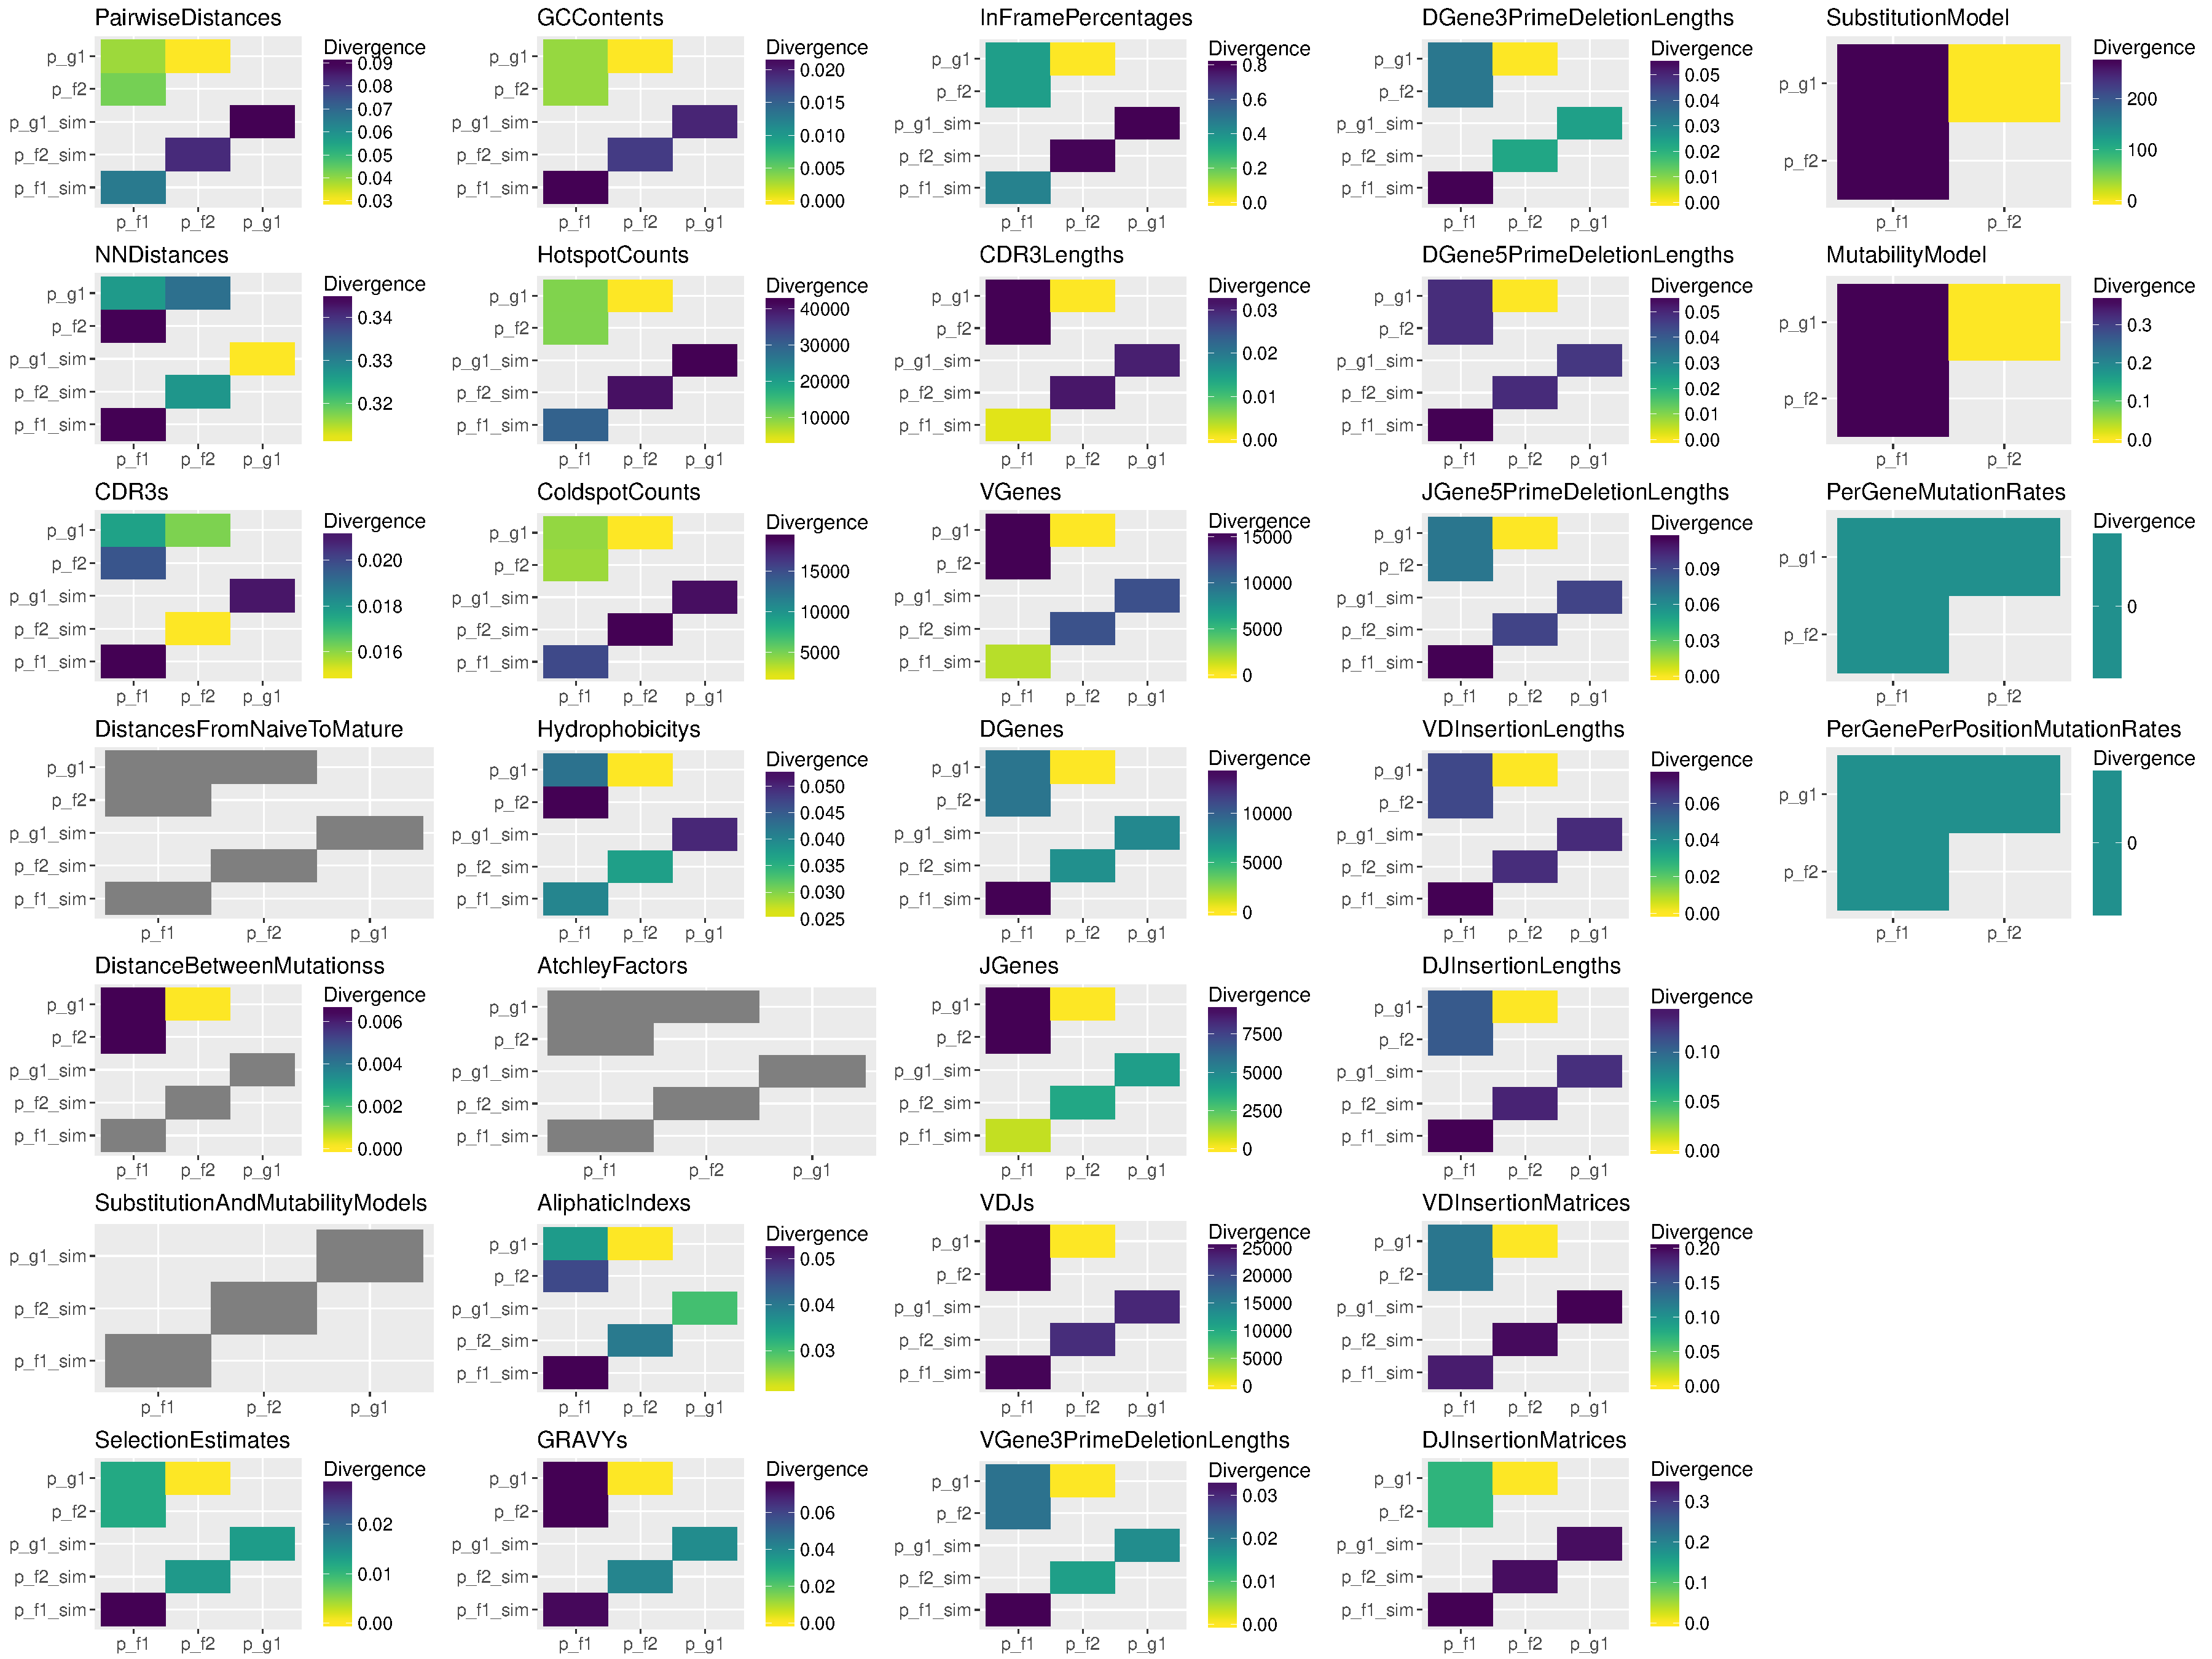
\includegraphics[width=\linewidth]{Figures/sim_obs.pdf}
    \caption{Divergences of empirical summary distributions based on three individual observed datasets.}
    \label{SimObs}
\end{figure}

\begin{figure}
    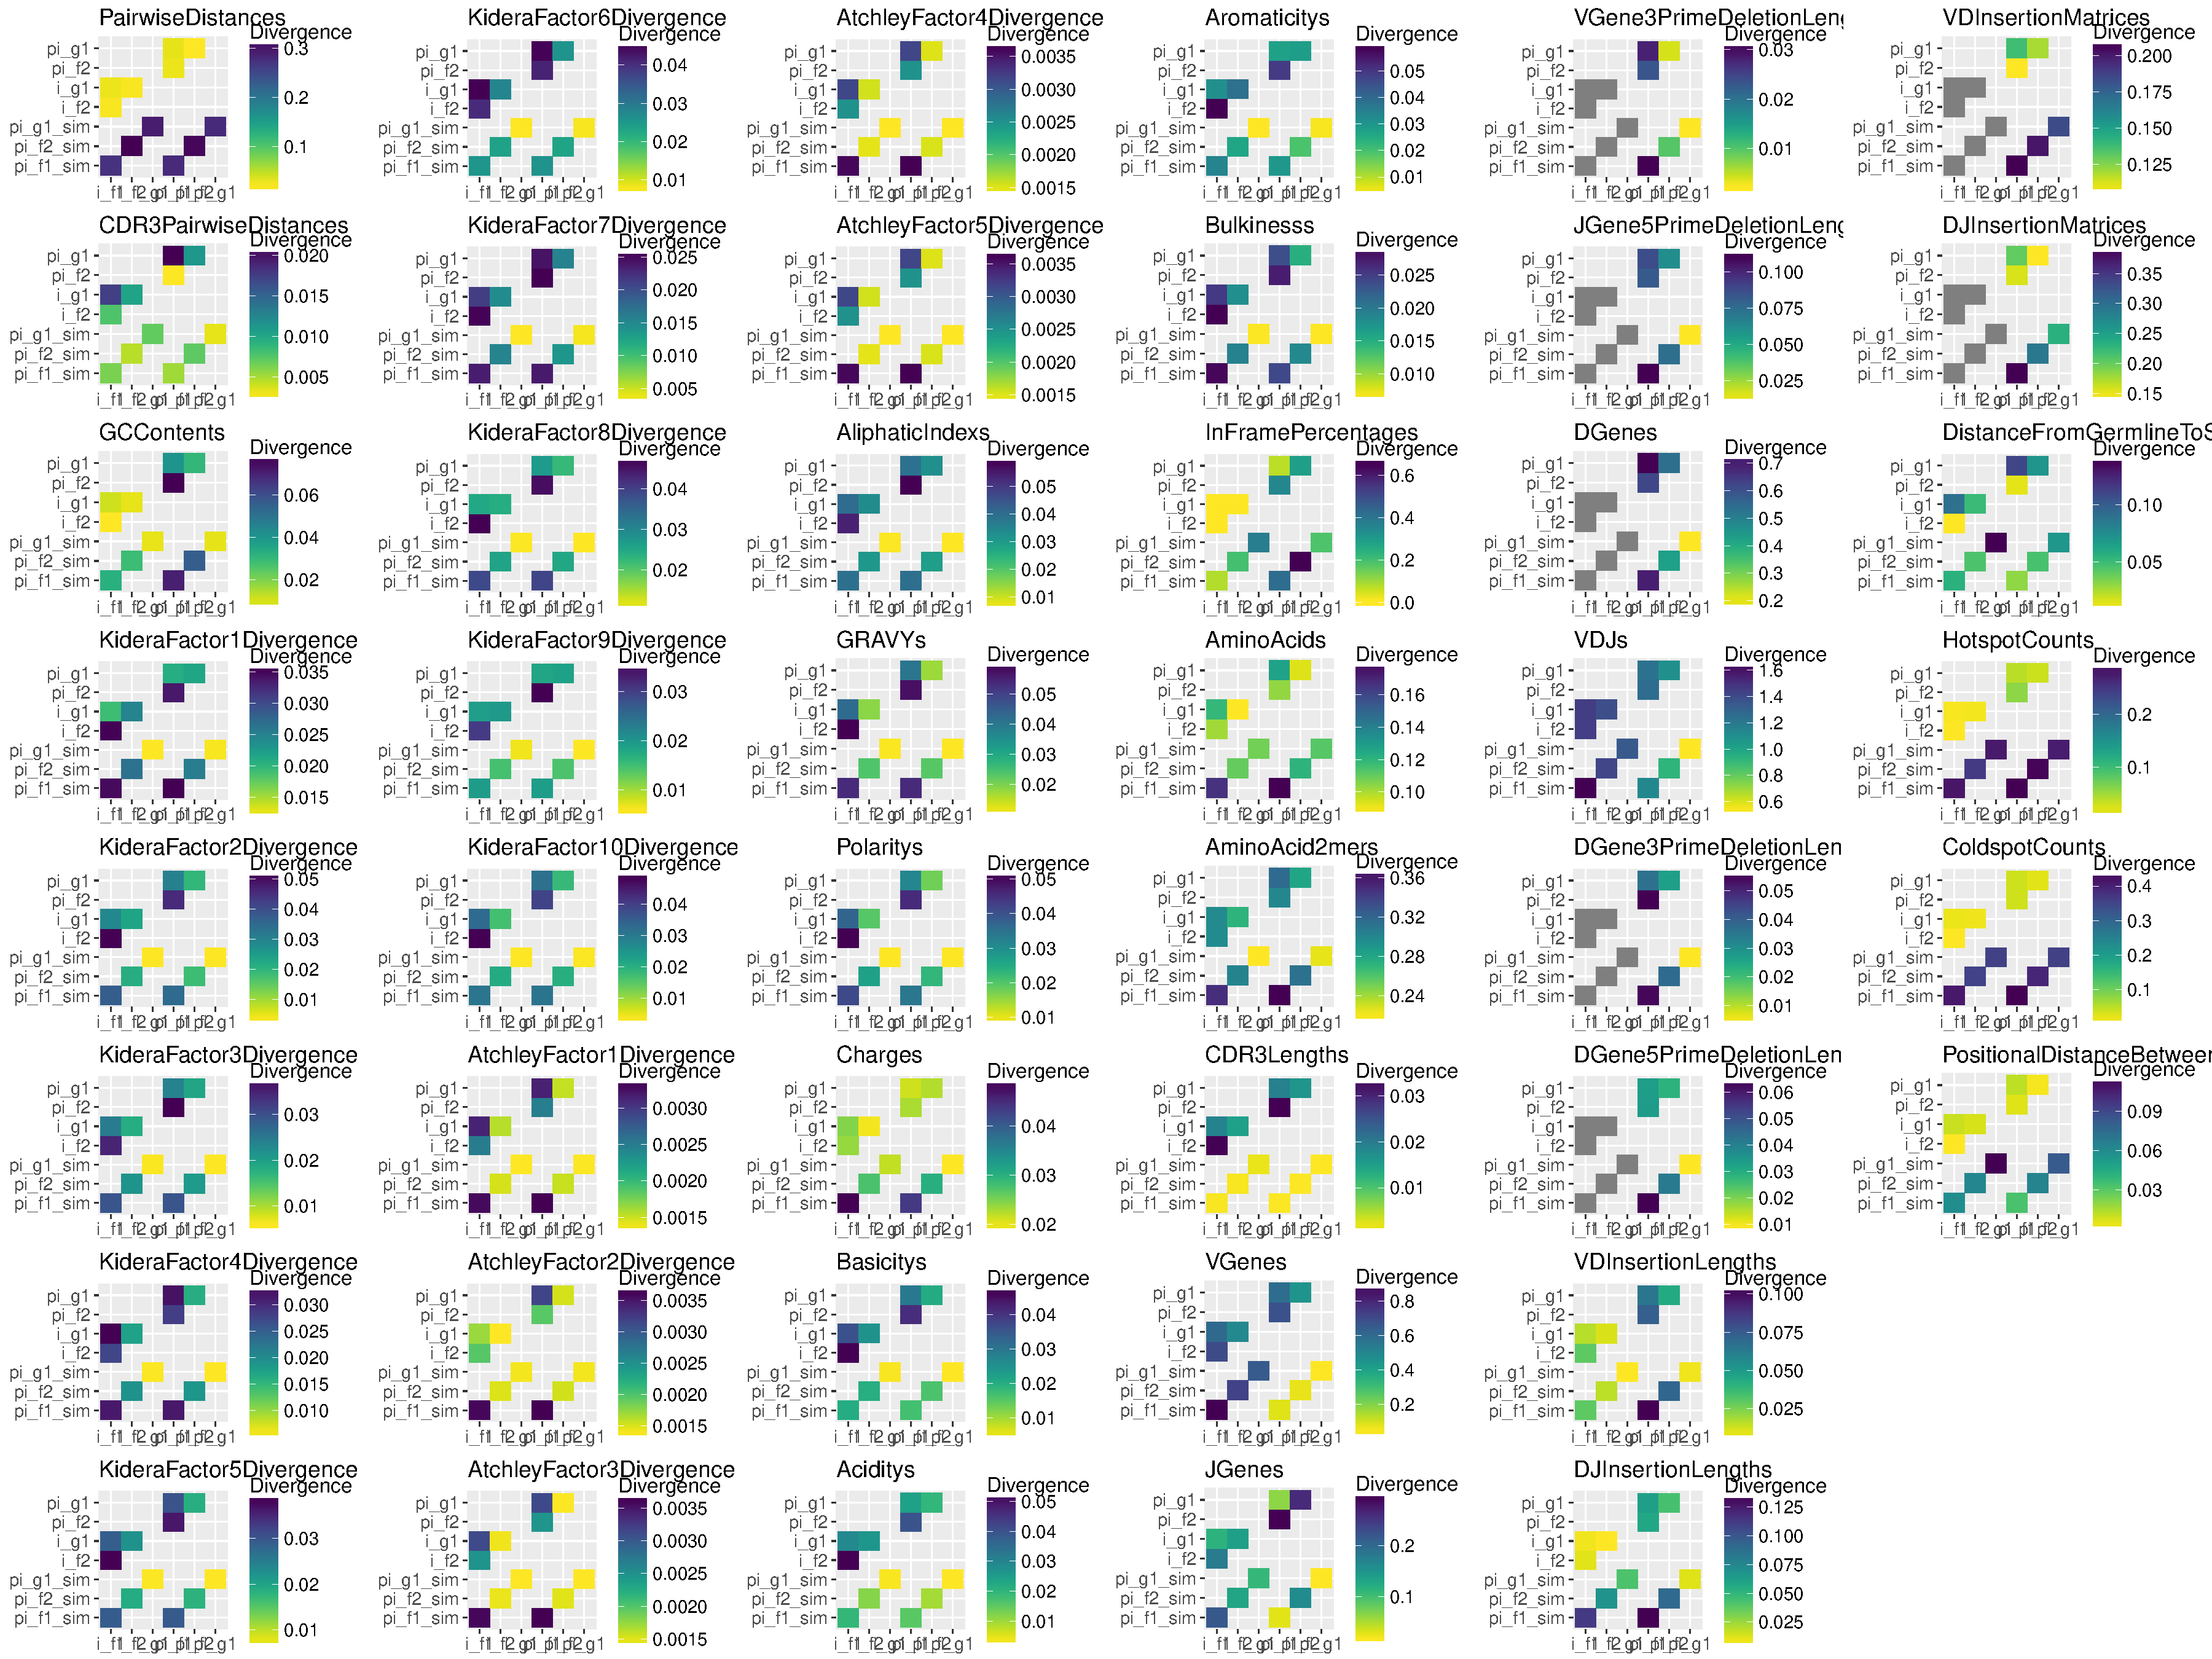
\includegraphics[width=\linewidth]{Figures/partis_igb.pdf}
\end{figure}

\begin{figure}
    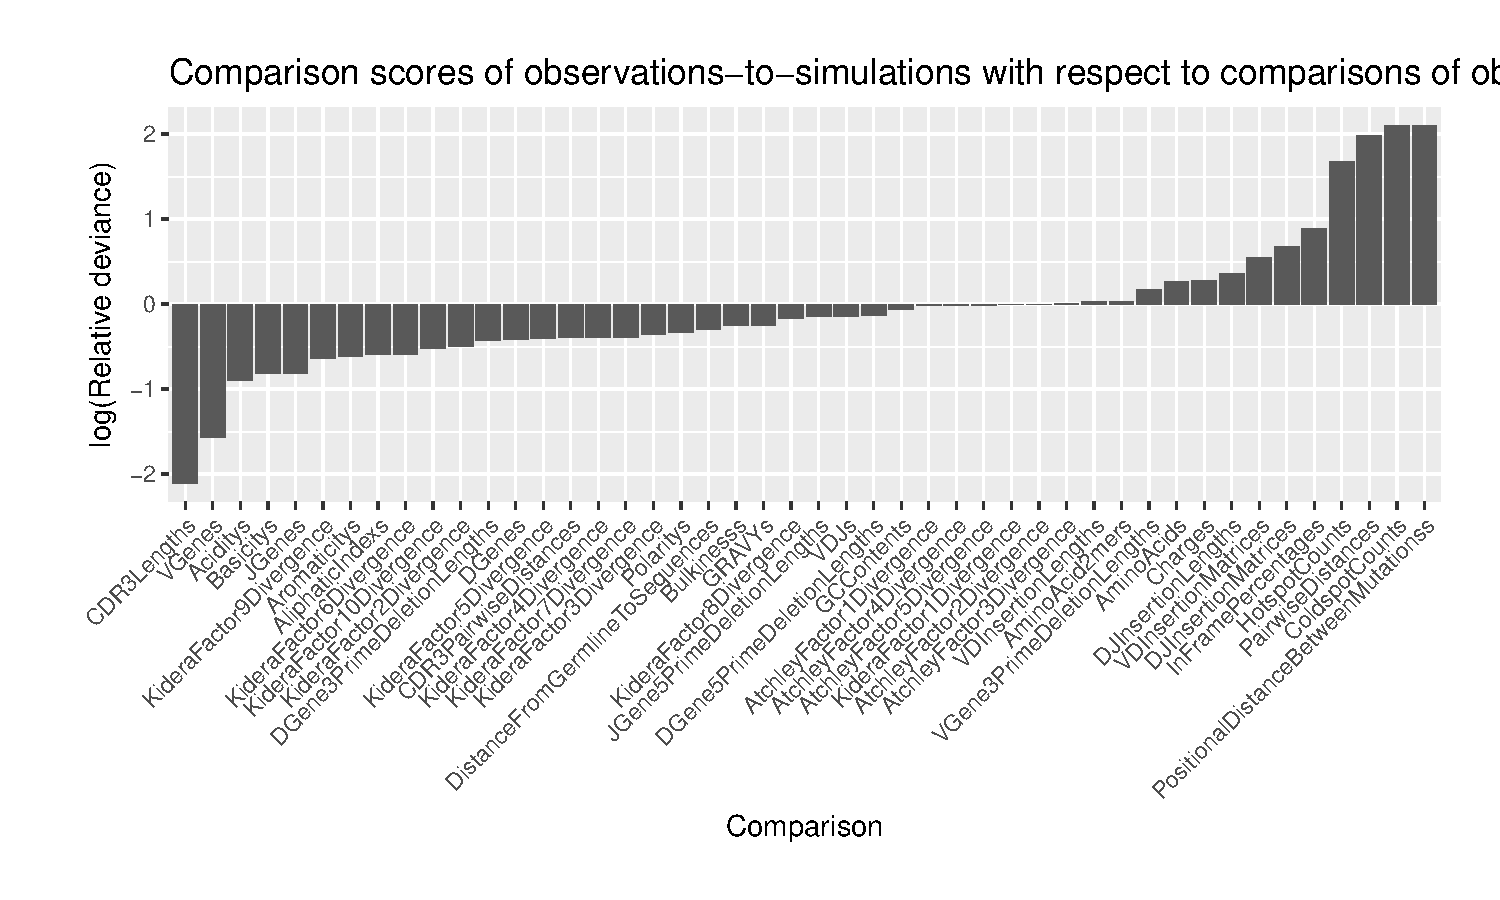
\includegraphics[width=\linewidth]{Figures/score_plot.pdf}
\end{figure}

\subsection*{Assessing summary statistic replication by model}

\subsection*{Comparing observations to competing model simulations}

\section{Discussion}
We aren't talking about pairwise summary statistics such as UniFrac \cite{De_Bourcy2017-pu}.


\bibliographystyle{plain}
\bibliography{main}

\end{document}
